\documentclass[twocolumn]{article}
\usepackage{cite}
\usepackage{hyperref}
\usepackage{graphicx}

\title{\textbf{Mapping the Intellectual Structure of Social Network Research: A Bibliometric Analysis of Three Journals}}
\author{\textbf{Pengjia Cui}}

\begin{document}
	
	\maketitle
	
	\begin{abstract}
		This study presents a comprehensive bibliometric analysis of research published in three leading journals in the field of social network studies: \textit{Social Networks}, \textit{Journal of Complex Networks}, and \textit{Network Science}. Using data retrieved from the \textit{Web of Science} (WoS), we employ performance analysis, science mapping, and network analysis to examine the intellectual structure, research trends, and collaboration patterns within the domain. Our findings reveal key thematic clusters, influential publications, and evolving research trajectories. Additionally, we assess the impact of prolific authors and institutions while mapping co-authorship networks to understand patterns of scholarly collaboration. By integrating multiple bibliometric techniques, this study provides a structured overview of the field’s development, offering insights into emerging research areas and future directions in social and complex network studies.
	\end{abstract}
	
	\section{Introduction}\label{Introduction}
	
	Bibliometric analysis provides a systematic approach to understanding the intellectual landscape and research dynamics within a scientific field. By examining publication and citation patterns, scholars can gain insights into key research themes, methodological trends, and the evolution of scholarly discourse. In this study, we conduct a bibliometric analysis of three leading journals in social and complex network research—\textit{Social Networks}, \textit{Journal of Complex Networks}, and \textit{Network Science}—to map the intellectual structure of the field, identify key themes and trends, assess research impact, and analyze collaboration patterns.
	
	Specifically, this study aims to: (1) map the intellectual structure of social network research by examining citation networks and scholarly influences, (2) identify key themes and trends by analyzing keyword co-occurrence and thematic clusters across the three journals, (3) assess research impact by evaluating citation counts, influential publications, and contributions from prolific authors and institutions, and (4) analyze collaboration patterns by exploring co-authorship networks and institutional affiliations.
	
	To achieve these objectives, our analysis is structured into three main components. First, we conduct a performance analysis to assess publication trends, citation impact, and the contributions of leading scholars and institutions. Second, we implement science mapping techniques—including co-citation analysis, bibliographic coupling, and keyword co-occurrence analysis—to explore the thematic evolution and intellectual structure of the field. Finally, we perform a network analysis to examine collaboration patterns among researchers, institutions, and countries, uncovering structural properties of co-authorship and citation networks.
	
	By integrating these approaches, this study offers a structured overview of the current research landscape in social and complex network studies. While not exhaustive, it provides valuable insights into the development and diffusion of knowledge in the field, highlighting emerging research trajectories and potential future directions.
	
	Having defined the aims and scope of this study, the next step is to determine the bibliometric techniques that will allow us to systematically analyze the research landscape within \textit{Social Networks}, \textit{Journal of Complex Networks}, and Network Science. Following \cite{donthu_how_2021}, we categorize our approach into three primary analytical components: performance analysis, science mapping, and network analysis. Each technique is selected to directly align with our research objectives.
	
	\section{Bibliometric Techniques}\label{Bibliometric Techniques}
	
	To systematically analyze the intellectual structure of social network research, this study employs three interconnected bibliometric approaches: performance analysis, science mapping, and network analysis. Each method offers distinct yet complementary insights into the research landscape of the three selected journals.
	
	\textbf{Performance analysis} provides a quantitative assessment of research productivity and impact by examining publication trends, citation metrics, and the contributions of influential authors, institutions, and countries.
	
	\textbf{Science mapping} uncovers the thematic and conceptual structure of the field by identifying research clusters, keyword co-occurrence patterns, and intellectual influences through co-citation and bibliographic coupling analyses.
	
	\textbf{Network analysis} explores patterns of collaboration among authors, institutions, and countries, shedding light on the social and structural dynamics of knowledge production in social network research.
	
	By systematically integrating these three analytical components, this study provides a comprehensive and structured overview of social network research across the selected journals. The results will:
	
	\begin{itemize}
		\item Reveal historical and emerging research trends, highlighting shifts in dominant themes and methodological approaches.
		\item Identify key contributors and influential works, offering insights into the most impactful papers, prolific scholars, and leading institutions.
		\item Map collaborative networks, examining how scholars, institutions, and countries interact and contribute to the field.
	\end{itemize}
	
	Our multi-faceted approach ensures that the study not only quantifies research impact but also contextualizes the development of ideas, theories, and methodologies in social network research. The following sections describe each bibliometric technique in detail, outlining its purpose, methodology, data requirements, and analytical tools.
	
	\section{Performance Analysis}\label{Performance Analysis}
	
	Performance analysis in bibliometrics provides an overview of research productivity, citation impact, and contributions of authors, institutions, and countries. It helps quantify the most influential publications, prolific researchers, and overall research trends in \textit{Social Networks}, \textit{Journal of Complex Networks}, and \textit{Network Science}.
	
	\subsection{Data Collection and Preprocessing}
	
	We use data retrieved from Web of Science (WoS), ensuring that only publications from the selected journals are included by filtering records based on their respective journal names and excluding any unrelated titles while removing all records with missing values. . The full query link are put below: 
	\begin{itemize}
		\item \url{https://www.webofscience.com/wos/woscc/summary/8b9cb9e7-5920-4a8c-8957-1f45746eb38f-01449729f7/relevance/1}
		\item 	\url{https://www.webofscience.com/wos/woscc/summary/b70d5df8-5cd9-4064-8329-390221e5fcc0-014497387b/relevance/1}
		\item 	\url{https://www.webofscience.com/wos/woscc/summary/cfb2985d-4457-4214-85c1-4ee6224ffecb-014497425b/relevance/1}
	\end{itemize}
	
	\subsection{Publication Trends in Social Network Research}
	
	\begin{figure}[htbp]
		\caption{Publication Trend}\label{fig.fig1}
		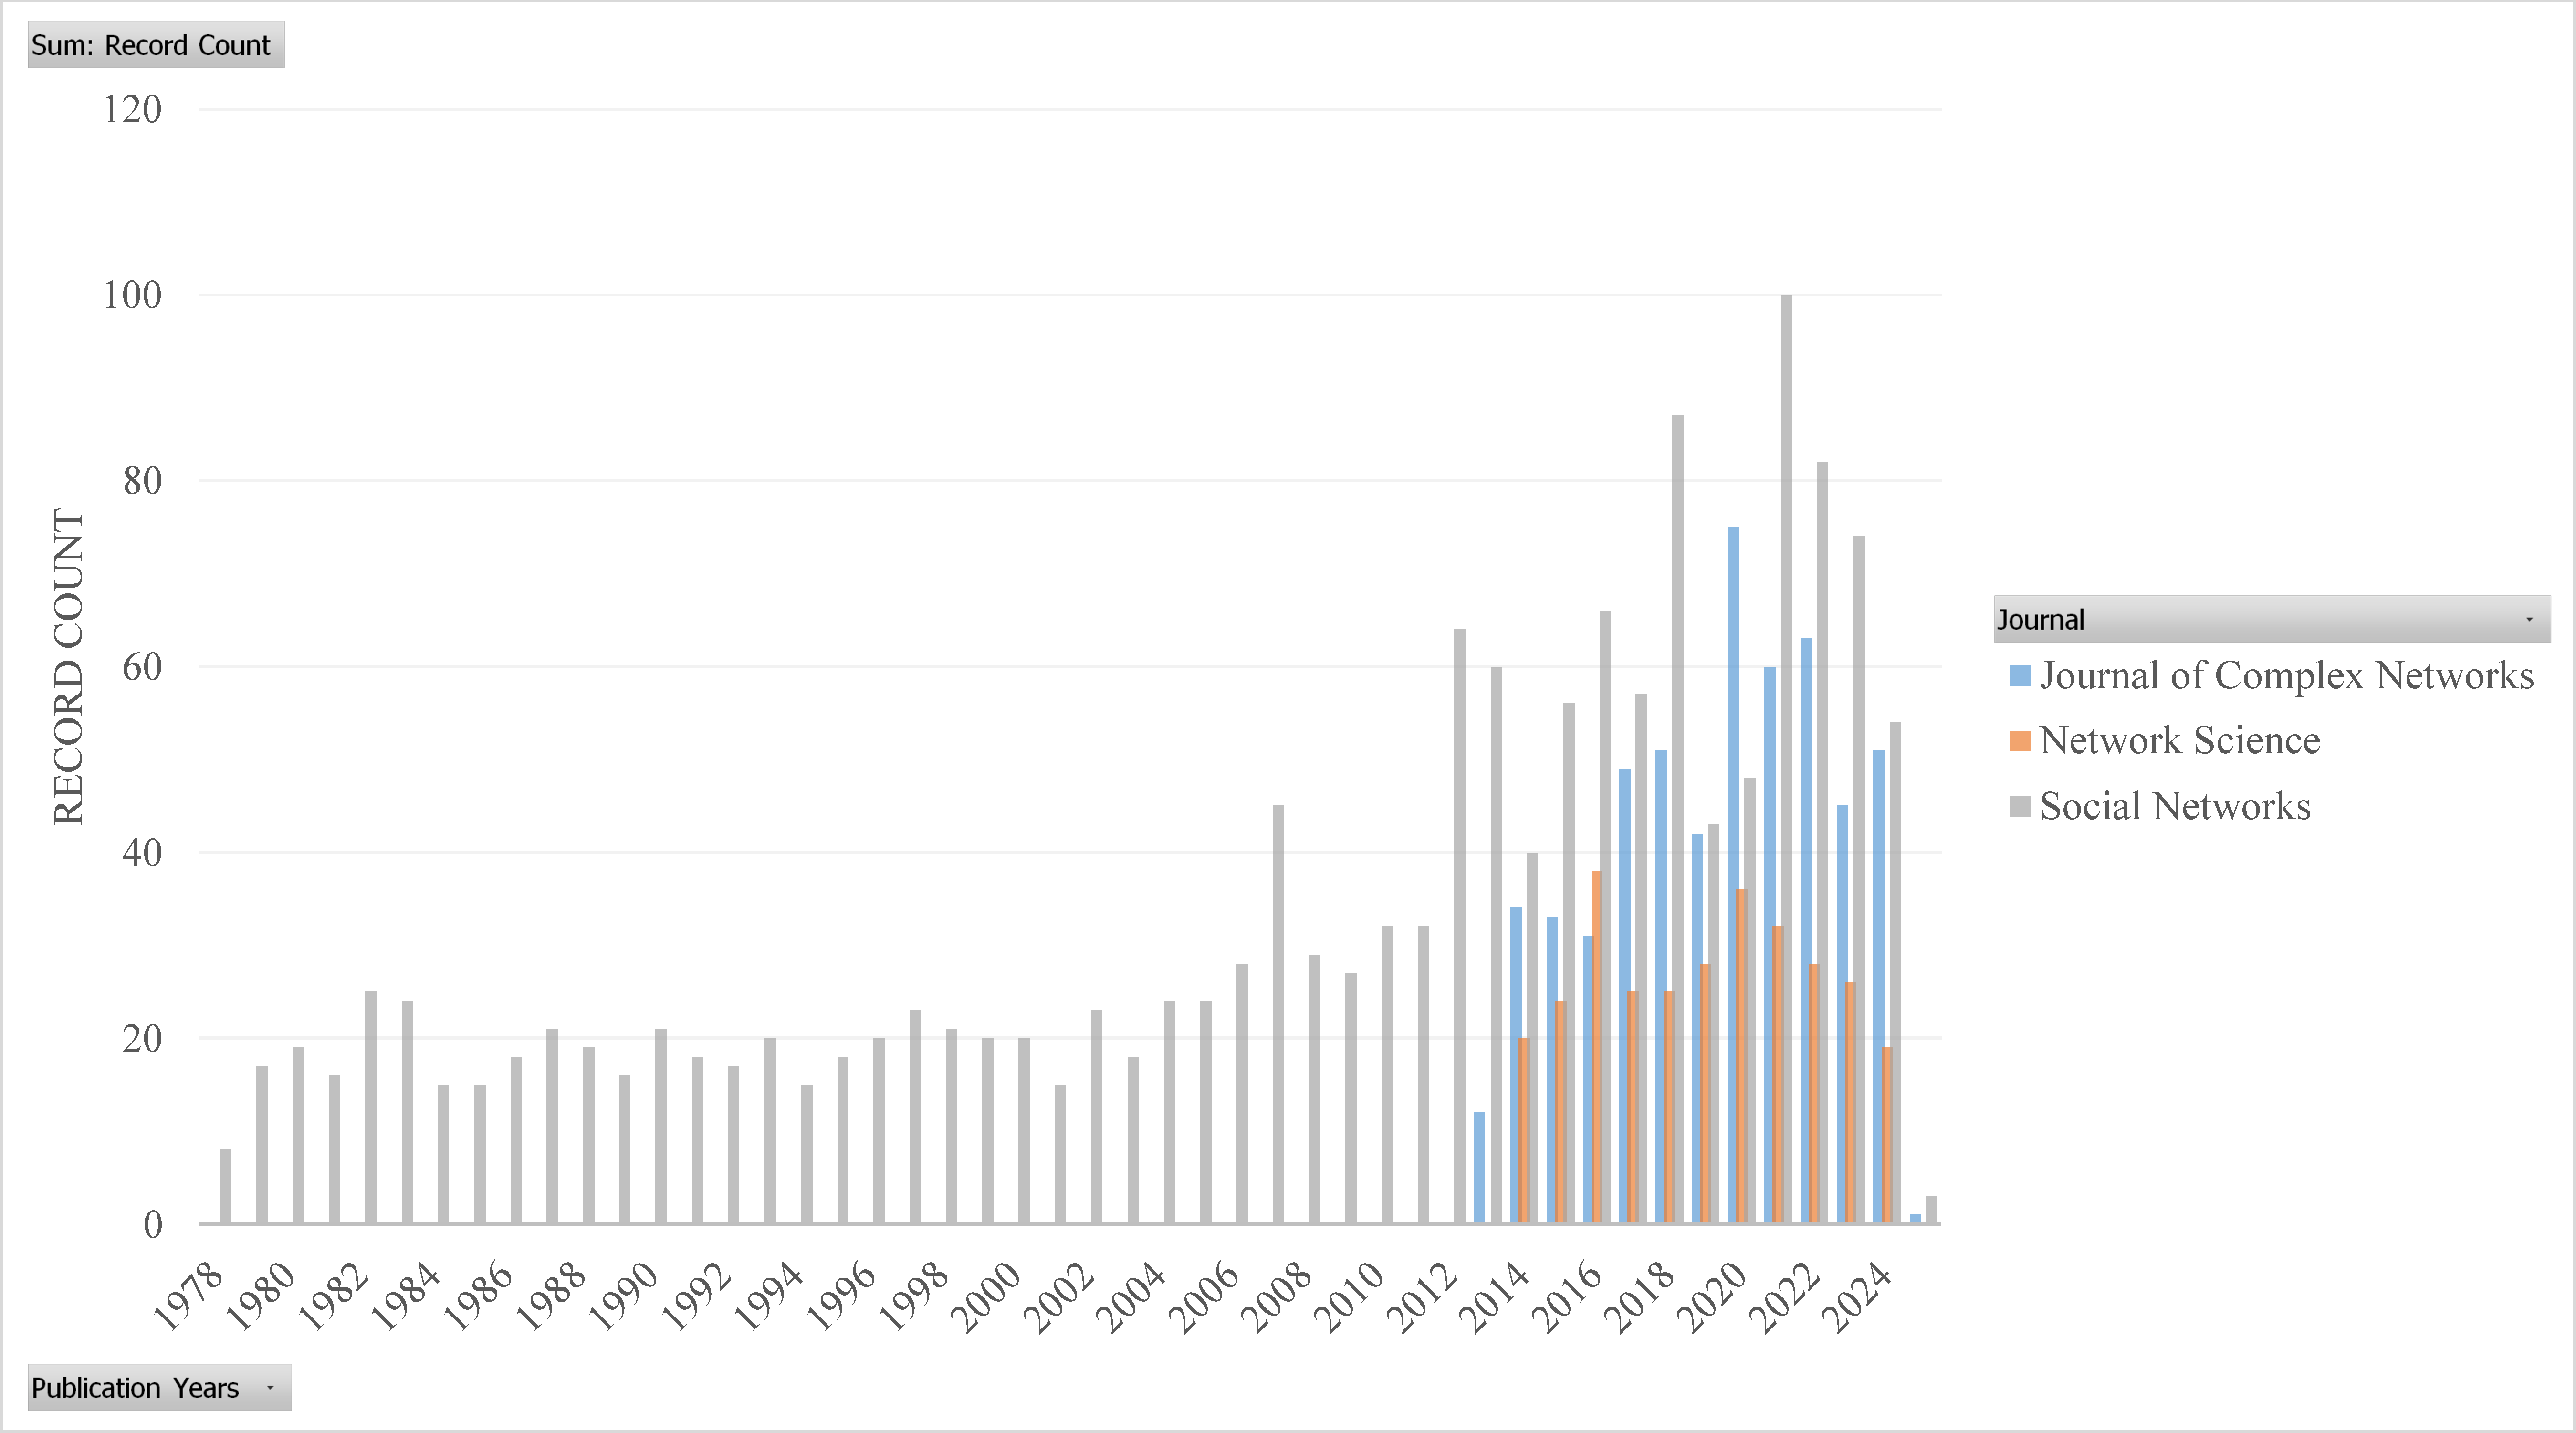
\includegraphics[width=\linewidth]{images/Record Count Proportion.pdf}
	\end{figure}
	
	This section analyzes the publication trends in three leading social network research journals as shown in Figure \ref{fig.fig1}. By examining their historical trajectories, we highlight the evolution of research output in the field and the emergence of specialized venues for network studies.
	
	\begin{enumerate}
		\item \textbf{The Dominance of Social Networks} \\
		As the oldest and most established journal in the field, Social Networks has consistently published research since its inception in 1978. For several decades, it was the primary outlet for studies on social network analysis. From 1978 to the early 2010s, its publication volume remained relatively stable, with moderate fluctuations. However, starting around 2010, the journal experienced a significant increase in output, peaking in the early 2020s. This surge reflects the growing prominence of computational and empirical approaches to network analysis.
		\item 	\textbf{The Emergence of Journal of Complex Networks} \\
		The establishment of Journal of Complex Networks in 2013 marked an expansion of the field, particularly in the study of mathematical and computational models of networks. Initially, its publication volume was low, but by 2015, the journal exhibited rapid growth. By 2020, its annual output was comparable to that of Social Networks, indicating that complex network research had developed into a distinct subfield with its own specialized audience.
		\item 	\textbf{Network Science as a Specialized Journal} \\
		Network Science, launched in 2014, has a comparatively lower publication volume than the other two journals. This suggests that it may cater to a more theoretical or interdisciplinary audience, focusing on foundational principles of network theory rather than applied studies. While its publication count has gradually increased, it remains the smallest of the three journals in terms of research output.
		\item 	\textbf{Growth and Peak Publication Years (2018–2022)} \\
		Between 2016 and 2022, all three journals saw a marked increase in publication volume, reflecting the rising academic interest in network science. Social Networks exceeded 100 publications per year, while Journal of Complex Networks and Network Science followed a similar trajectory, albeit at a lower scale. This period corresponds to the expansion of big data research, computational social science, and machine learning applications, all of which have influenced network studies.
		
		\item \textbf{Recent Decline or Stabilization (Post-2022)} \\
		In the most recent years (2023–2024), a decline in publication counts is observed. However, this may be attributed to:
		
		\begin{itemize}
			\item Incomplete indexing of recent publications in databases.
			\item A genuine stabilization of research output after years of rapid growth. Further analysis is needed to determine whether this trend reflects a saturation of the field or a shift in research priorities.
		\end{itemize}
		
	\end{enumerate}
	
	The trends observed across these three journals suggest the institutionalization and diversification of social network research:
	
	\begin{itemize}
		\item \textbf{Social Networks} remains the core journal for traditional social network studies.
		\item \textbf{Journal of Complex Networks} has emerged as a venue for computational and mathematical approaches.
		\item \textbf{Network Science} occupies a specialized niche, potentially bridging different disciplines. Future analyses will examine citation impact, author collaboration networks, and thematic trends to better understand the intellectual structure and evolution of the field.
	\end{itemize}
	
	\subsection{Prolific Authors}
	
	In this analysis, we focus on identifying the most prolific authors in social network research based on their publication count across three key journals. By examining the record count for each author, we gain insights into the researchers who have made substantial contributions to the development of social network science. 
	
	\begin{figure}[htbp]
		\caption{Prolific Authors}\label{fig.fig2}
		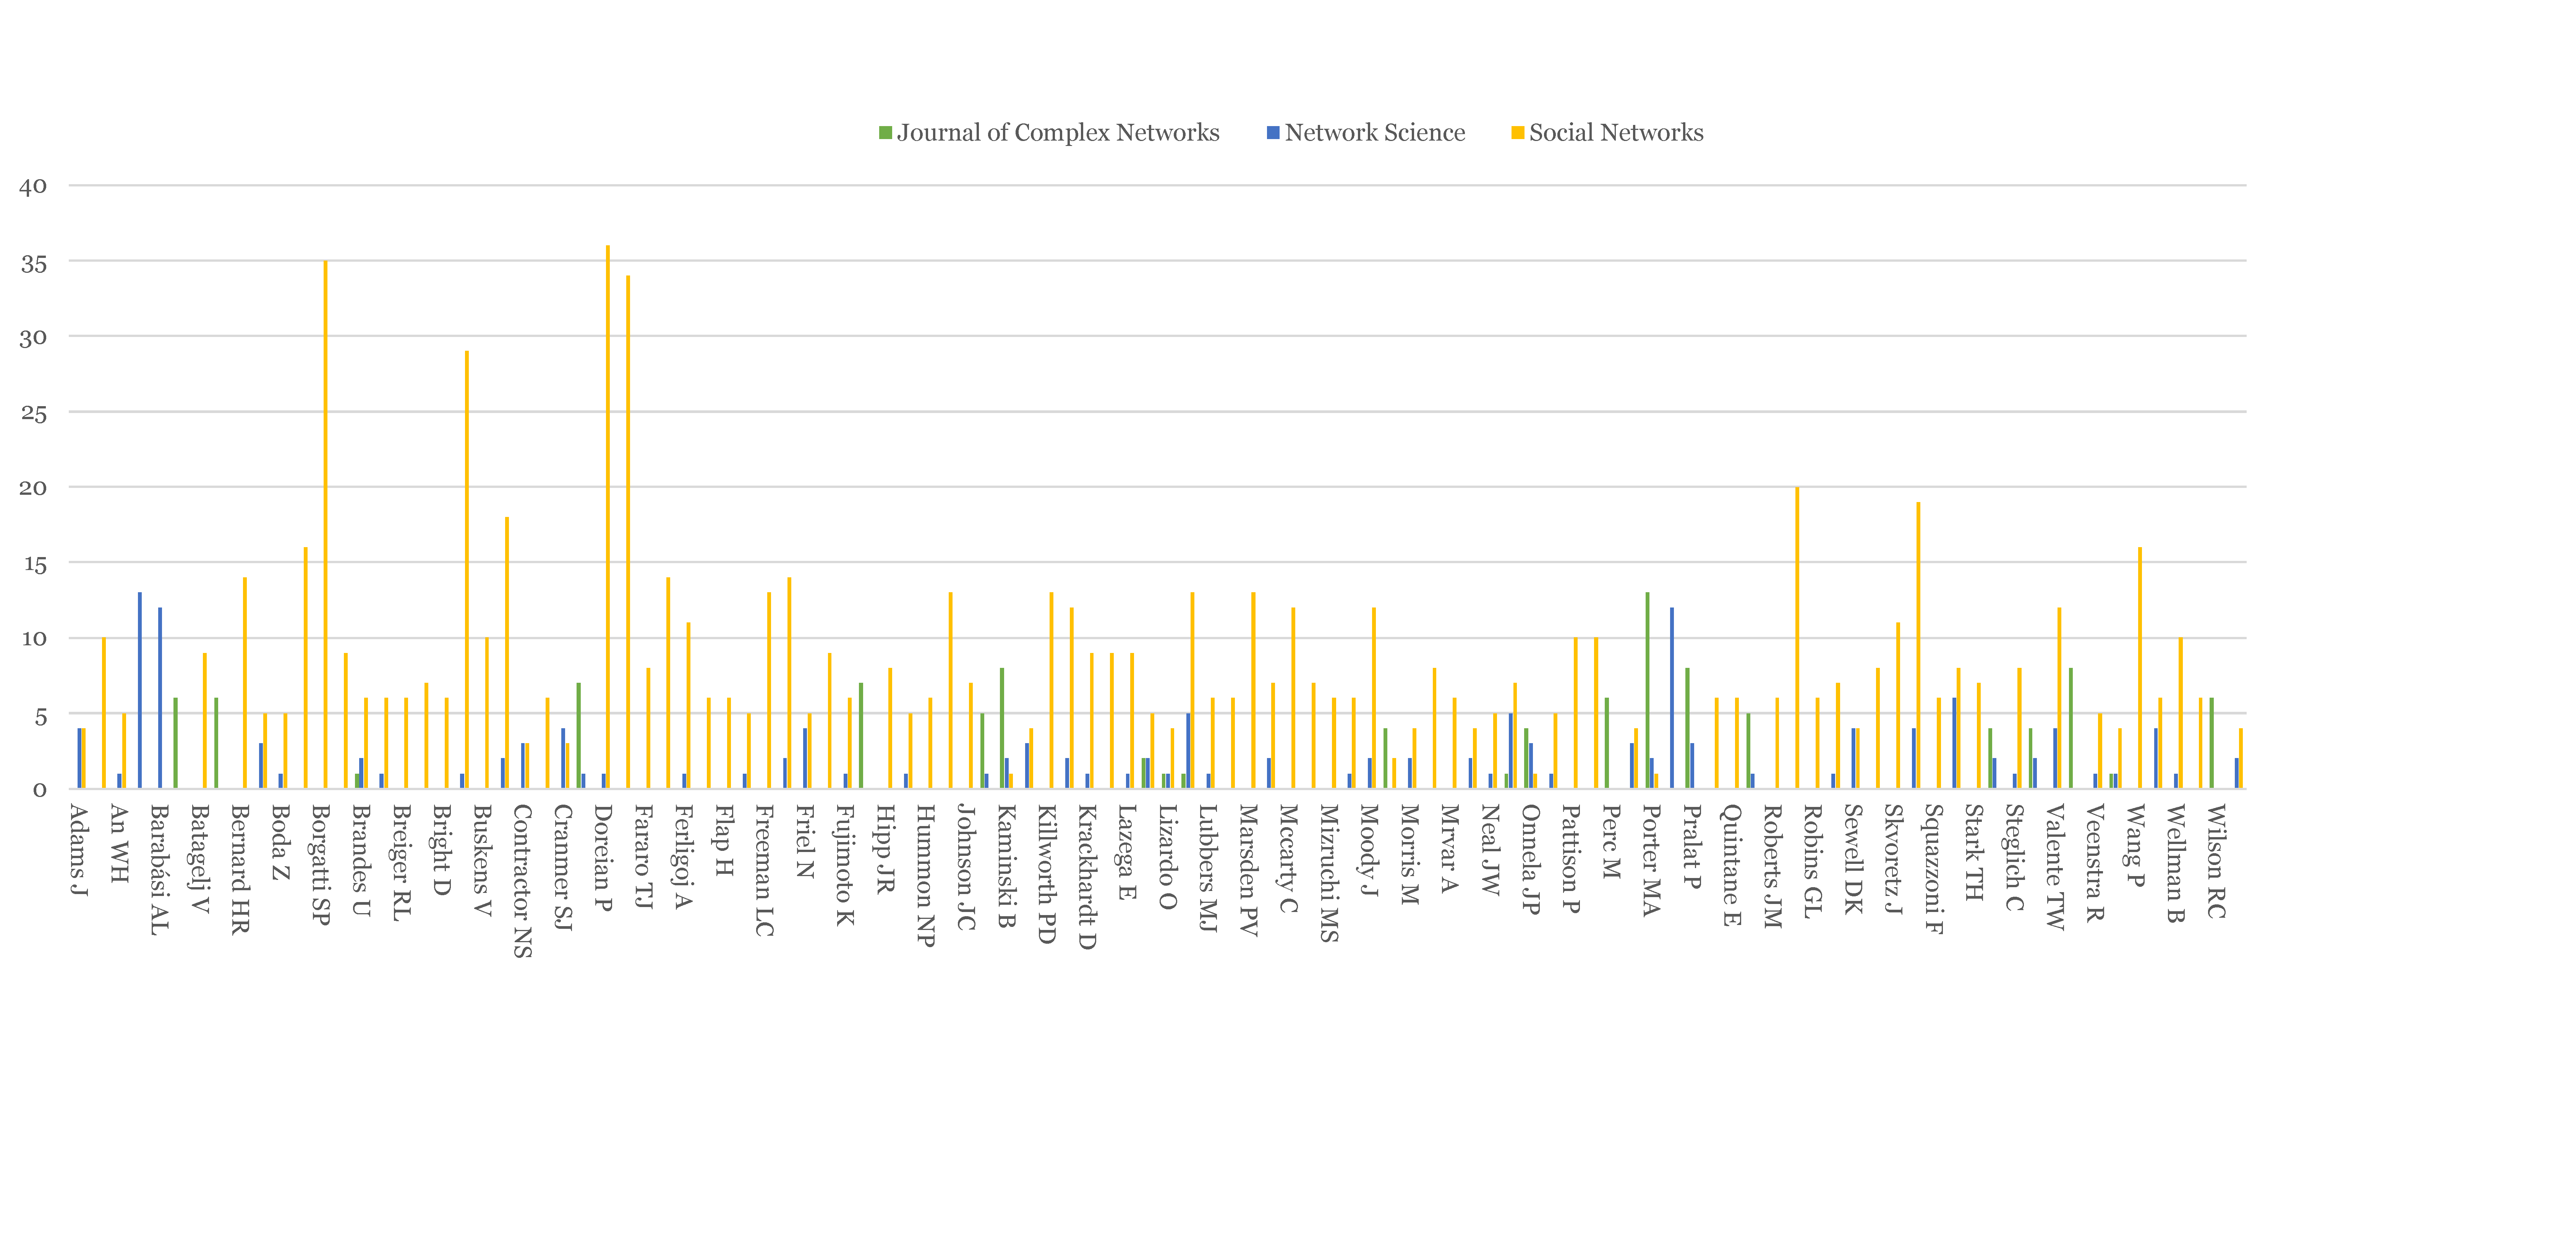
\includegraphics[width=\columnwidth]{images/Record Count of Top 100 Authors.pdf}
	\end{figure}
	
	The list of the top 100 authors reveals significant variation in their contributions to these journals. Authors with the highest record counts are likely to be the most influential thought leaders in the field. Their consistent productivity underscores their pivotal role in shaping the direction of social network research.

	\begin{enumerate}
		\item \textbf{Leading Authors:} \\ The authors with the top publication counts are those who have actively contributed to multiple research topics and have seen consistent growth in their academic output. These prolific authors have published across various subfields of network science, demonstrating their versatility and importance in the research community.
		\item \textbf{Journal Contributions:}
		\begin{itemize}
			\item Social Networks remains the dominant venue for many authors, reflecting its longstanding influence in the field. Authors contributing to this journal tend to focus on applied social network analysis, sociology, and related disciplines.
			\item Journal of Complex Networks and Network Science attract authors working in the mathematical, computational, and interdisciplinary aspects of network theory. These journals are increasingly popular among authors exploring complex network models, algorithmic approaches, and theoretical research.
		\end{itemize}
		\item \textbf{Distribution of Publications:} \\ The proportion of publications across journals offers insight into the shifting focus of social network research. While many top authors have a balanced publication record across journals, others specialize in specific areas. Some authors are heavily concentrated in Network Science or Journal of Complex Networks, indicating a deeper engagement with theoretical and computational network studies.
	\end{enumerate}

	By identifying the most prolific authors, this analysis provides a snapshot of the academic leaders driving the research agenda in social network science. Their work has not only contributed to the growth of the field but has also helped establish the intellectual foundations that connect different branches of network theory and applications.
	
	These findings are important for understanding how individual contributions have shaped the evolution of social network research. In particular, the comparison of publication output across journals provides insight into the interdisciplinary nature of the field and the distinct but complementary research focuses of Social Networks, Journal of Complex Networks, and Network Science.
	
	\bibliographystyle{apalike}
	\bibliography{ref}
	
\end{document}
